\documentclass[10pt]{article}
\usepackage[utf8]{inputenc}
\usepackage[T1]{fontenc}
\usepackage{amsmath}
\usepackage{amsfonts}
\usepackage{amssymb}
\usepackage[version=4]{mhchem}
\usepackage{stmaryrd}
\usepackage{graphicx}
\usepackage[export]{adjustbox}
\graphicspath{ {./images/} }

\begin{document}
\begin{enumerate}
  \item By calculating the limit
\end{enumerate}

$$
\lim _{h \rightarrow 0} \frac{f(x+h)-f(x)}{h}
$$

find the derivatives of the following functions at $x=a$ :\\
(a) $f(x)=\frac{1}{x}$ for $a \neq 0$.\\
(b) $f(x)=\sqrt{x}$ for $a \neq 0$.\\
(c) $f(x)=\frac{1}{\sqrt{x}}$ for $a \neq 0$.\\
(d) $f(x)=x^{3}-3 x+5$.\\
(e) $f(x)=x^{1 / 4}$.\\
(f) ${ }^{*} f(x)=\sin \left(x^{2}\right)$.\\[0pt]
[Hint: For (f) you can use that as $h$ approaches $0, \sin h \approx h$ and $\cos h \approx 1-h^{2}$ ]

\section*{GROUP WORK 1, SECTION 2.7}
Follow that Car\\
The distance travelled by a car is given by $d(t)=8\left(t^{3}-6 t^{2}+12 t\right)$, where $d$ is in miles and $t$ is in hours.

\begin{enumerate}
  \item Draw a graph of $d(t)$ from $t=0$ to $t=3$.
  \item Does the car ever stop?
  \item What is the average velocity over $[1,3]$ ? over $[1.5,2.5]$ ? over $[1.9,2.1]$ ?
  \item Estimate the instantaneous velocity at $t=2$. Give a physical interpretation of your answer.
  \item We know that $d(t)=8\left(t^{3}-6 t^{2}+12 t\right)$\\
now factorize $=8 t\left(\frac{\left.t^{2}-6 t+12\right)}{}\right.$
\end{enumerate}

$$
\begin{aligned}
& d(0)=0 \\
& d(1)=52 \\
& d(2)=64 \\
& d(3)=72
\end{aligned}
$$

$b^{2}-4 a c<0$ so has no roots

$$
t^{2}-6 t+12=(t-3)^{2}+3
$$

complete the\\
square\\
so its graph looks like\\
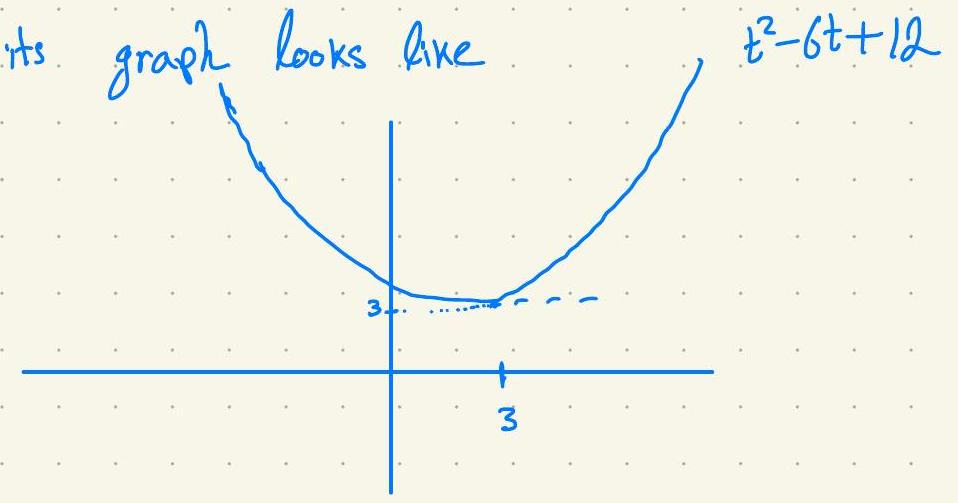
\includegraphics[max width=\textwidth, center]{2024_12_26_646789e1ccd1e87aeca8g-03}

So the graph of $8 t\left(t^{2}-6 t+12\right)$ should look like\\
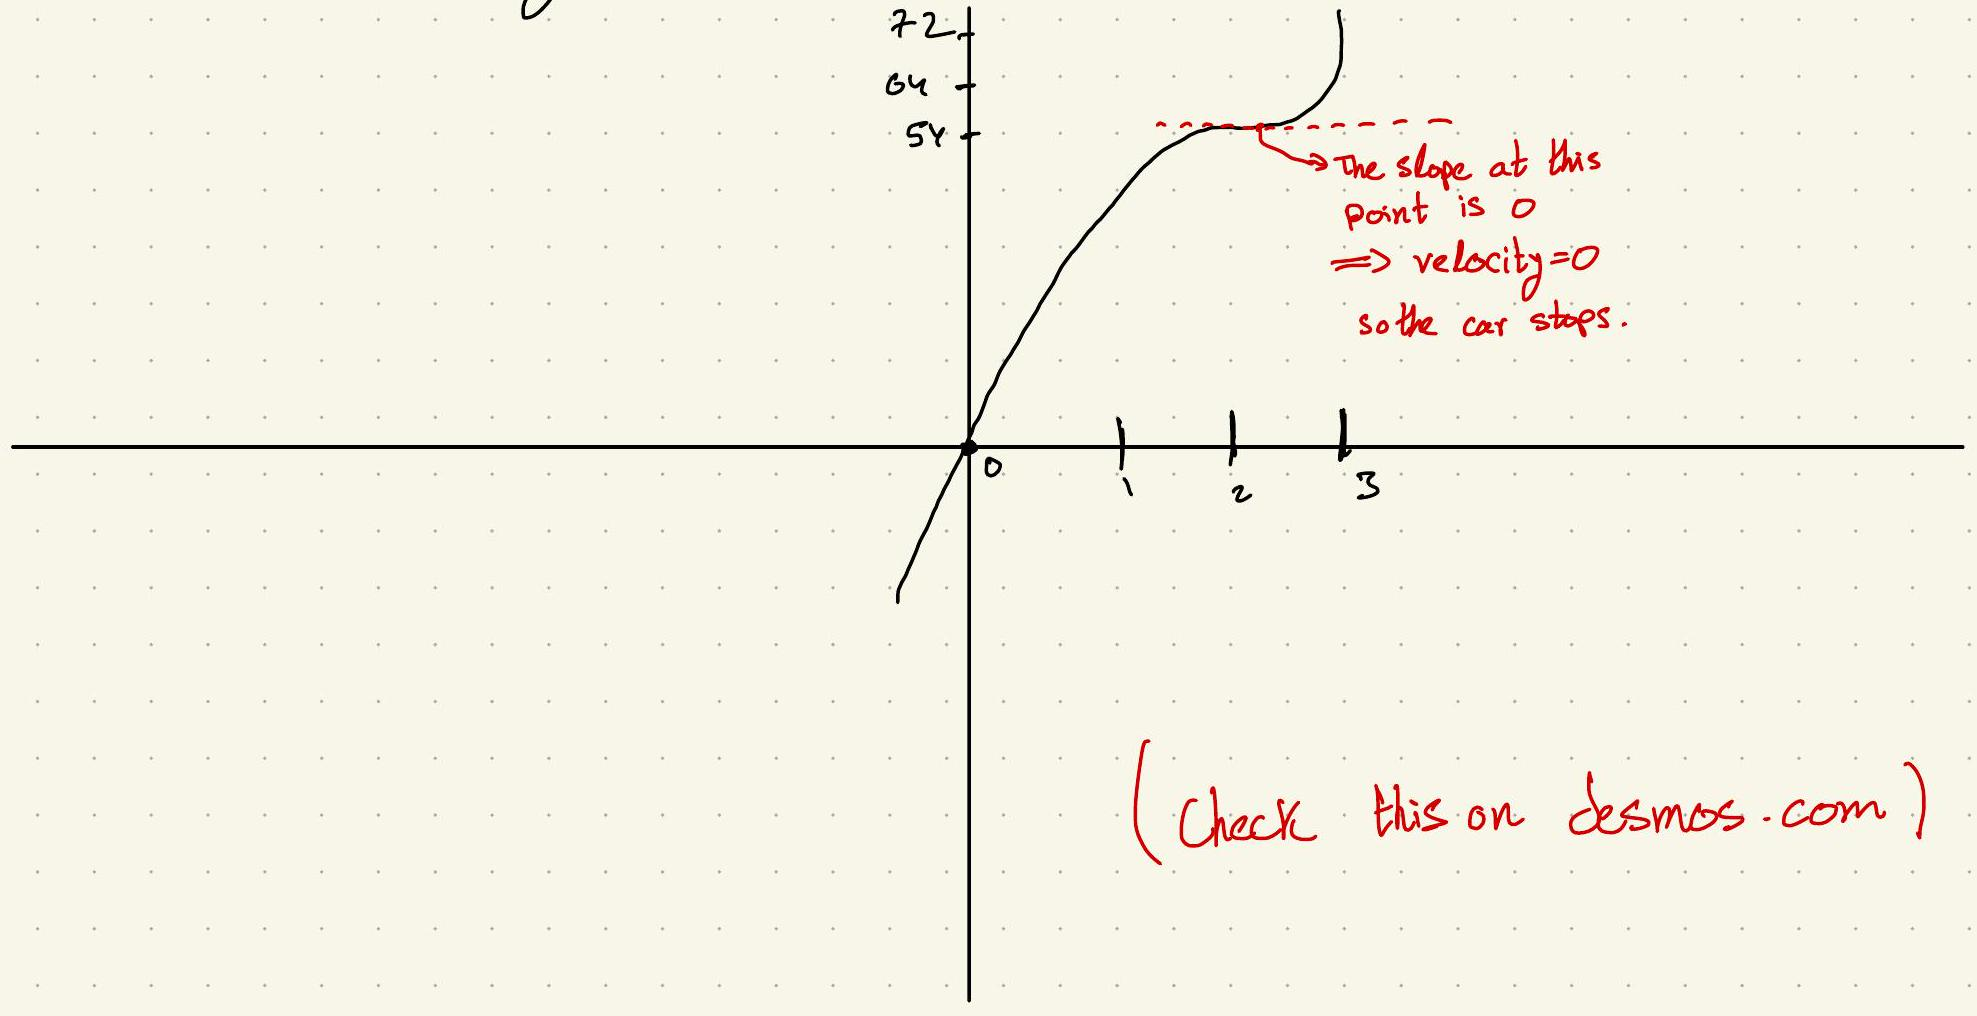
\includegraphics[max width=\textwidth, center]{2024_12_26_646789e1ccd1e87aeca8g-03(1)}\\
3.

$$
\begin{aligned}
\text { average velocity } & =\frac{\Delta \text { distance }}{\Delta \text { time }} \\
\text { - on }[1,3]: \Delta \text { distance } & =\partial(3)-\partial(0)=20 \\
\Delta \text { time } & =3-1=2 \\
\text { average velocity } & =\frac{20}{2}=10 \text { miles/hour }
\end{aligned}
$$

\begin{itemize}
  \item On $[1.5,2.5]: \quad \Delta$ distance $=\partial(2.5)-d(1.5)=2$\\
$\Delta$ time $=2.5-1.5=1$\\
average velocity $=\frac{2}{1}=2$ miles/ how
  \item Or $[1.9,2]: \Delta$ distance $=\partial(21)-\partial(1.9)=0.016$\\
$\Delta$ time $=21-1.9=0.2$
\end{itemize}

$$
\text { average velocity }=\frac{0.016}{0.2}=0.8 \text { miles/hour }
$$

Looks like as we get closer to $t=2$, the average velocity approaches $\mathcal{O}$. So the instantaneous velocity at $t=2$ is omiles /hour. That means the car stops momentarily.

\section*{Connect the Dots}
A company does a study on the effect of production value $p$ of an advertisement on its consumer approval rating $A$. After interviewing eight focus groups, they come up with the following data:

\begin{center}
\begin{tabular}{|c|c|}
\hline
Production Value & Consumer Approval \\
\hline
$\$ 1000$ & $32 \%$ \\
$\$ 2000$ & $33 \%$ \\
$\$ 3000$ & $46 \%$ \\
$\$ 3500$ & $55 \%$ \\
$\$ 3600$ & $61 \%$ \\
$\$ 3800$ & $65 \%$ \\
$\$ 4000$ & $69 \%$ \\
$\$ 5000$ & $70 \%$ \\
\hline
\end{tabular}
\end{center}

Assume that $A(p)$ gives the consumer approval percentage as a function of $p$.

\begin{enumerate}
  \item Estimate $A^{\prime}(\$ 3500)$. Is this likely to be an overestimate or an underestimate?
\end{enumerate}

We can estimate $A^{\prime}(3500) \cong \frac{A(3600)-A(3500)}{3600-3500}=\frac{61-55}{100}=0.07$\\
It looks like around 3500 , A is increasing at a decreasing rate and $3600>3500$\\
so this is likely an underestimate.\\
2. Interpret your answer to Problem 1 in real terms. What does your estimate of $A^{\prime}(\$ 3500)$ tell you? It means roughly that every $\$ 1$ of extra production value will increase consumer approval by $0.07 \%$\\
3. What are the units of $A^{\prime}(p)$ ?\\
It is \%/\$\\
4. Estimate $A^{\prime}(\$ 3550)$. Is your estimate better or worse than your estimate of $A^{\prime}$ (\$3500)? Why? Based on the information given, our best estimate is still 0.07 and we expect it to give a slightly better estimate since $A^{\prime}(3500)$ was likely an underestimate.

GROUP WORK 1, SECTION 2.8\\
Tangent Lines and the Derivative Function\\
The following is a graph of $g(x)=x \ln x$.\\
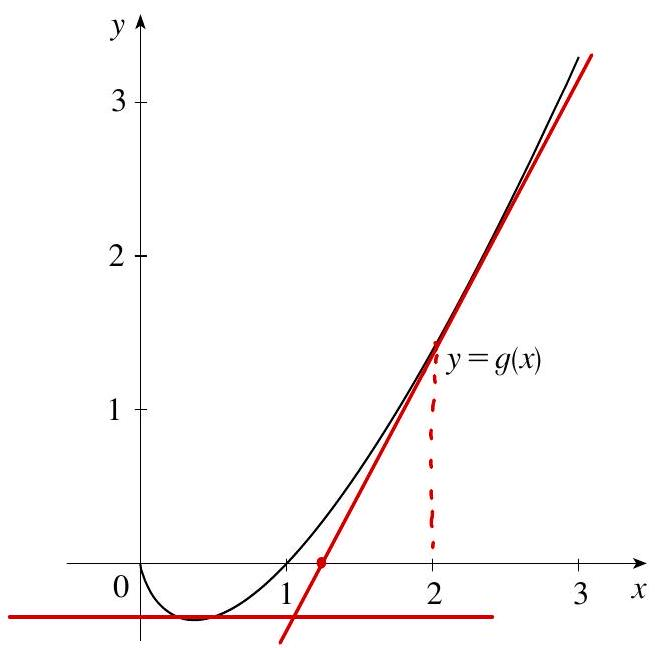
\includegraphics[max width=\textwidth, center]{2024_12_26_646789e1ccd1e87aeca8g-06}

It is a fact that the derivative of this function is $g^{\prime}(x)=\ln x+1$.

\begin{enumerate}
  \item Sketch the line tangent to $g(x)$ at $x=2$ on the graph above.
  \item Find an equation of the tangent line at $x=2$.\\
$g^{\prime}(2)=\ln (2)+1$ and $g(2)=2 \ln (2)$. So the live has slope $\ln (2)+1$ and passes through the point $(2,2 \ln (2))$. So it has equation
\end{enumerate}

$$
y=(\ln (2)+1) x-2
$$

\begin{enumerate}
  \setcounter{enumi}{2}
  \item Now sketch the line tangent to $g(x)$ at $x=\frac{1}{e} \approx 0.368$.
  \item Find an equation of the tangent line at $x=\frac{1}{e}$.
\end{enumerate}

Note: $\ln \left(\frac{1}{e}\right)=-\ln (e)=-1$.\\
This line has slope $g^{\prime}\left(\frac{1}{e}\right)=\ln \left(\frac{1}{e}\right)+1=0$ and passes through

$$
\left(\frac{1}{e}, g\left(\frac{1}{e}\right)\right)=\left(\frac{1}{e}, \frac{-1}{e}\right) \quad \text { so it has equation } y=\frac{-1}{e} \text {. }
$$

\section*{The Derivative Function}
The graphs of several functions $f$ are shown below. For each function, estimate the slope of the graph of $f$ at various points. From your estimates, sketch graphs of $f^{\prime}$.\\
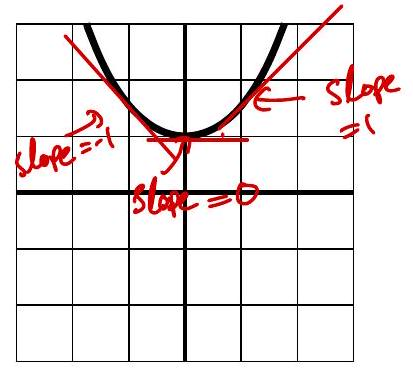
\includegraphics[max width=\textwidth, center]{2024_12_26_646789e1ccd1e87aeca8g-07(1)}

Graph 1\\
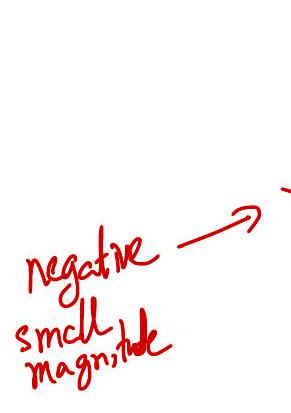
\includegraphics[max width=\textwidth, center]{2024_12_26_646789e1ccd1e87aeca8g-07}\\
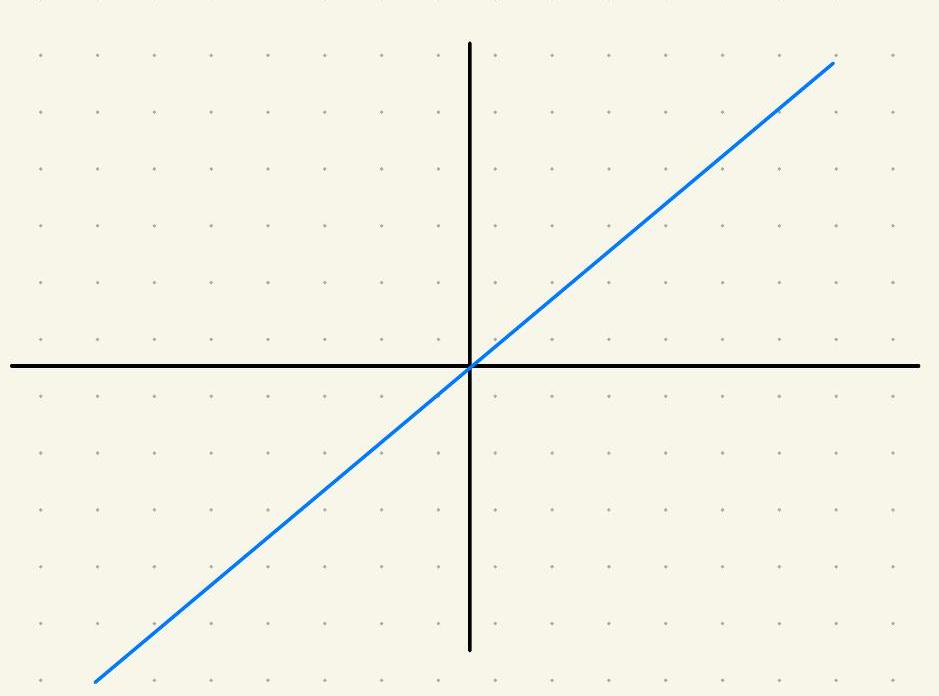
\includegraphics[max width=\textwidth, center]{2024_12_26_646789e1ccd1e87aeca8g-08}

Graph $f$\\
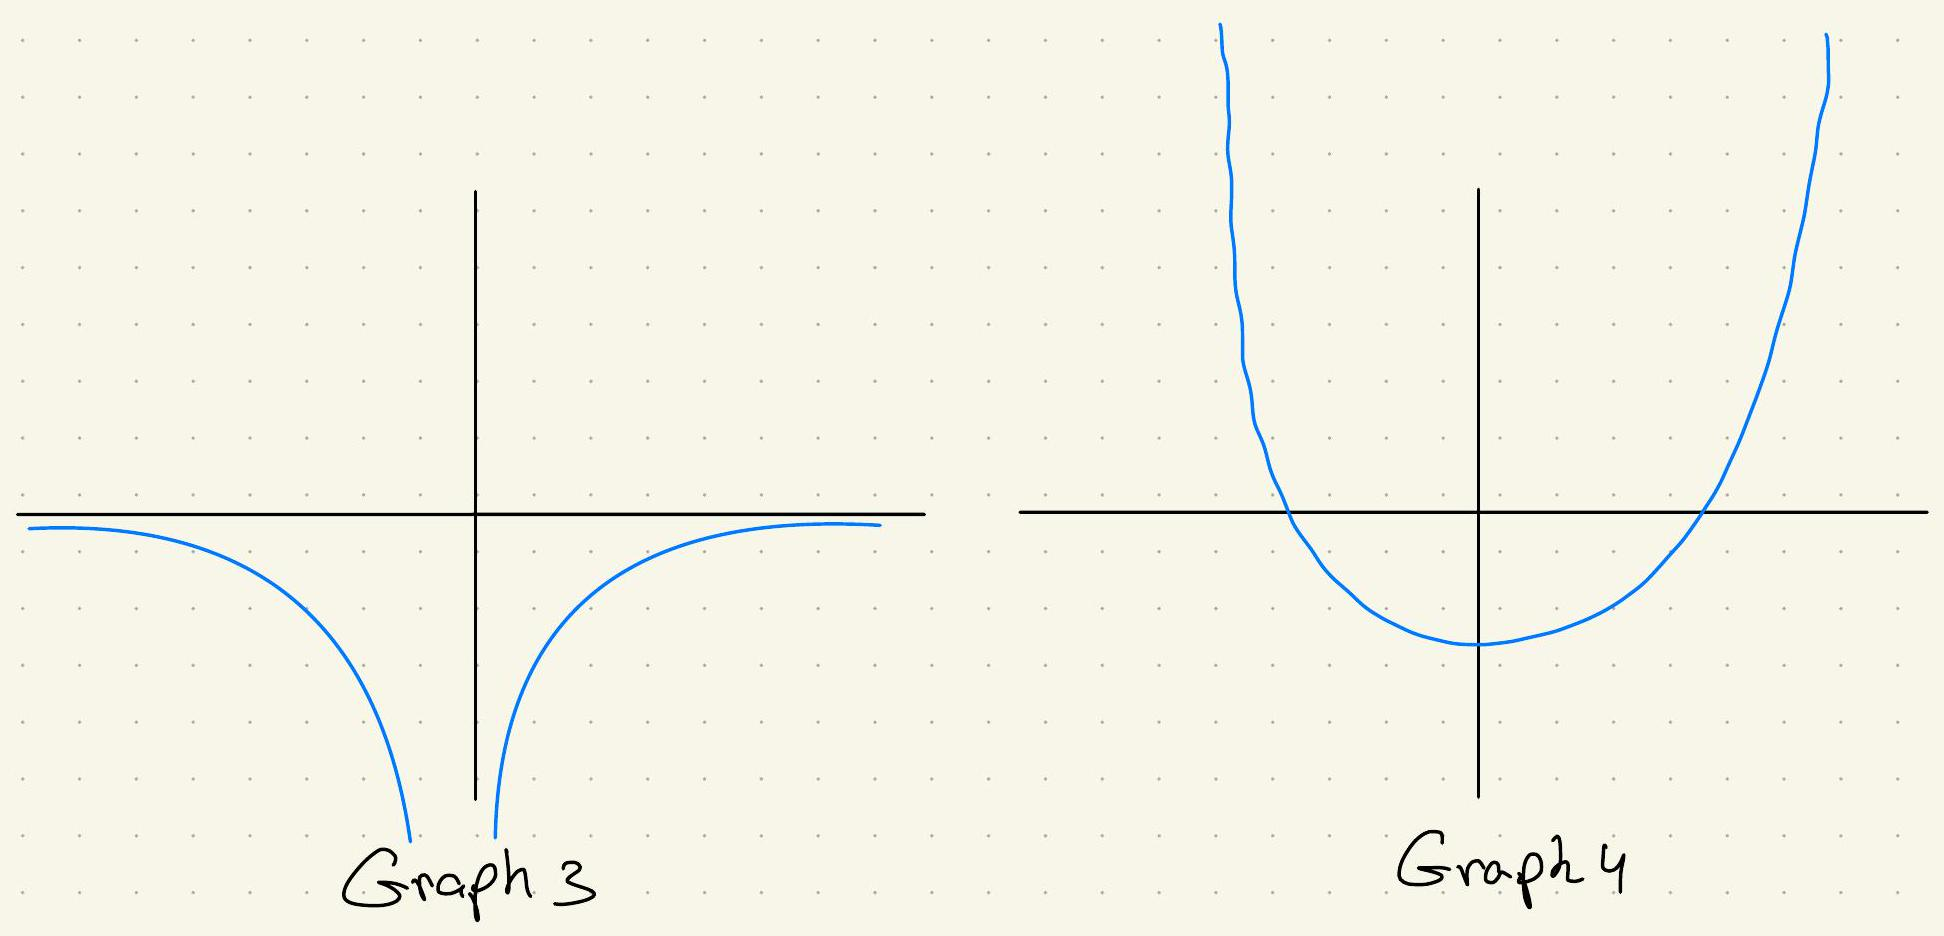
\includegraphics[max width=\textwidth, center]{2024_12_26_646789e1ccd1e87aeca8g-08(1)}\\
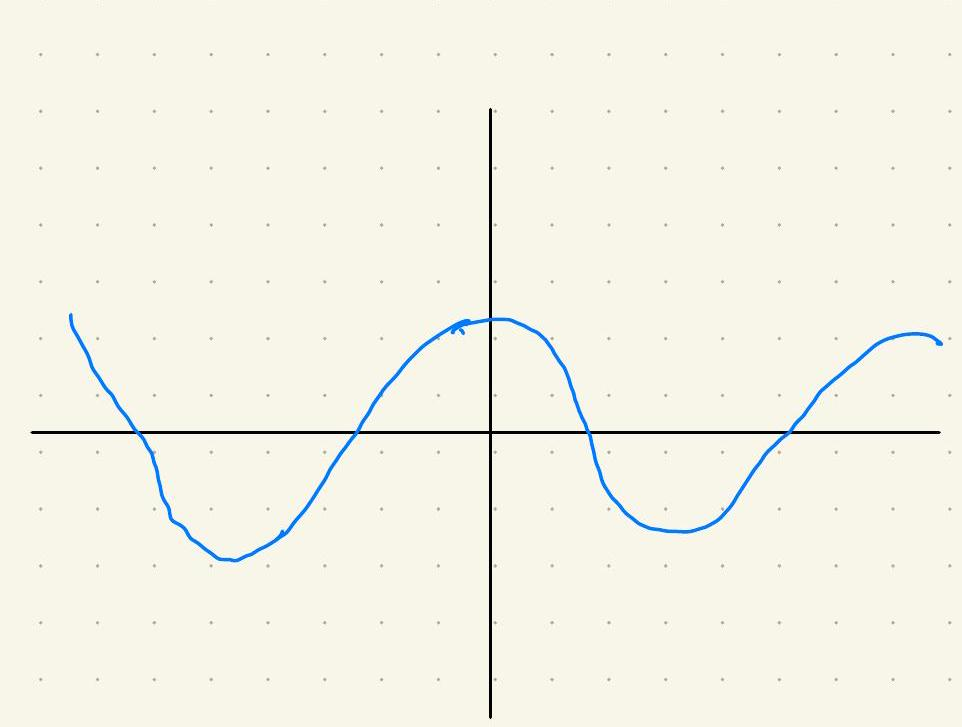
\includegraphics[max width=\textwidth, center]{2024_12_26_646789e1ccd1e87aeca8g-09(1)}

Graph 5\\
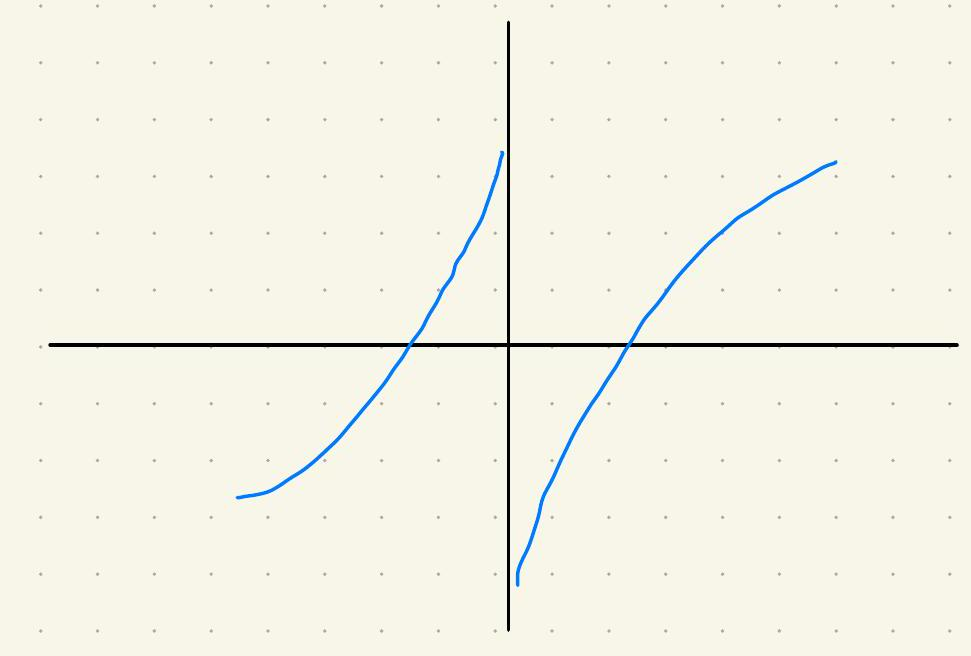
\includegraphics[max width=\textwidth, center]{2024_12_26_646789e1ccd1e87aeca8g-09(2)}

Graph 7\\
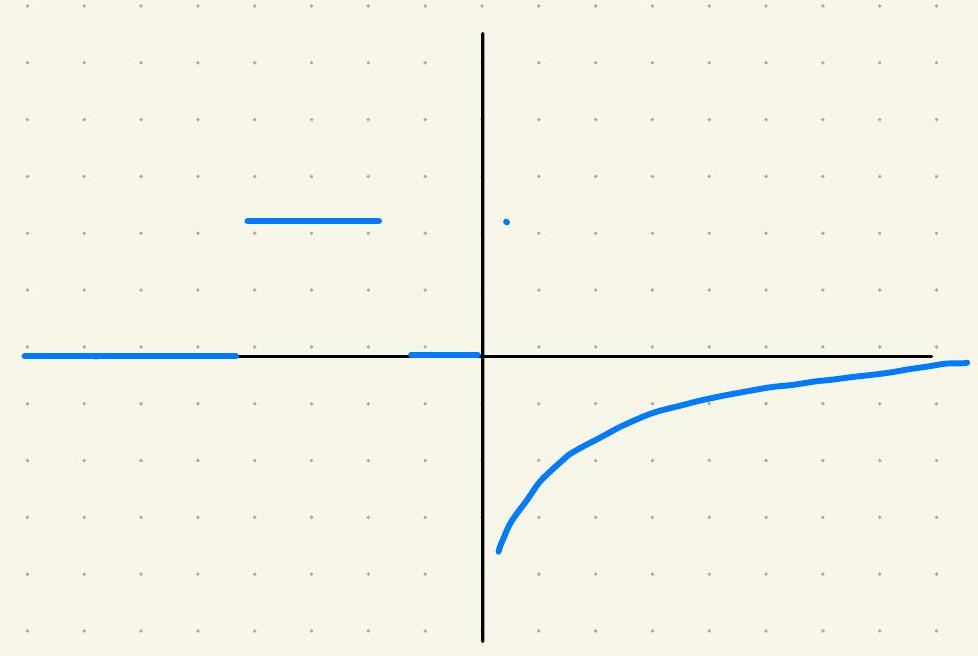
\includegraphics[max width=\textwidth, center]{2024_12_26_646789e1ccd1e87aeca8g-09}

Graph 8

\begin{enumerate}
  \item By calculating the limit
\end{enumerate}

$$
\lim _{h \rightarrow 0} \frac{f(a+h)-f(a)}{h}
$$

find the derivatives of the following functions at $x=a$ :\\
(a) $f(x)=\frac{1}{x}$ for $a \neq 0$.\\
(b) $f(x)=\sqrt{x}$ for $a \neq 0$.\\
(c) $f(x)=\frac{1}{\sqrt{x}}$ for $a \neq 0$.\\
(d) $f(x)=x^{3}-3 x+5$.\\
(e) $f(x)=x^{1 / 3}$.\\
(f) $f(x)=\sin \left(x^{2}\right)$.\\[0pt]
[Hint: For (f) you can use that as $h$ approaches $0, \sin h \approx h$ and $\cos h \approx 1-h^{2}$ ]

\section*{Solution}
(a)

$$
\lim _{h \rightarrow 0} \frac{\frac{1}{a+h}-\frac{1}{a}}{h}=\lim _{h \rightarrow 0} \frac{-h}{h a(a+h)}=\lim _{h \rightarrow 0} \frac{-1}{a(a+h)}=\frac{-1}{a^{2}}
$$

(b)

$$
\lim _{h \rightarrow 0} \frac{\sqrt{a+h}-\sqrt{a}}{h}
$$

multiply top and bottom by $\sqrt{a+h}+\sqrt{a}$ gives

$$
\lim _{h \rightarrow 0} \frac{h}{h(\sqrt{a+h}+\sqrt{a})}=\lim _{h \rightarrow 0} \frac{1}{\sqrt{a+h}+\sqrt{a}}=\frac{1}{2 \sqrt{a}}
$$

(c)

$$
\lim _{h \rightarrow 0} \frac{\frac{1}{\sqrt{a+h}}-\frac{1}{\sqrt{a}}}{h}=\lim _{h \rightarrow 0} \frac{\sqrt{a}-\sqrt{a+h}}{h \sqrt{a+h} \sqrt{a}}
$$

again, multiply top and bottom by $\sqrt{a}+\sqrt{a+h}$ gives

$$
\lim _{h \rightarrow 0} \frac{-h}{h \sqrt{a+h} \sqrt{a}(\sqrt{a+h}+\sqrt{a})}=\frac{-1}{2 \sqrt{a}^{3}}
$$

(d)

$$
\begin{gathered}
\lim _{h \rightarrow 0} \frac{(a+h)^{3}-3(a+h)+5-a^{3}+3 a-5}{h}=\lim _{h \rightarrow 0} \frac{3 a^{2} h+3 a h^{2}+h^{3}-3 h}{h}= \\
\lim _{h \rightarrow 0} 3 a^{2}+3 a h+h^{2}-3=3 a^{2}-3
\end{gathered}
$$

(e)

$$
\lim _{h \rightarrow 0} \frac{(a+h)^{1 / 4}-a^{1 / 4}}{h}
$$

Now multiply top and bottom by $(a+h)^{2 / 3}+(a+h)^{1 / 3} a^{1 / 3}+a^{2 / 3}$. This gives,


\begin{gather*}
\lim _{h \rightarrow 0} \frac{h}{h\left((a+h)^{2 / 3}+(a+h)^{1 / 3} a^{1 / 3}+a^{2 / 3}\right)}=\lim _{h \rightarrow 0} \frac{1}{(a+h)^{1 / 3} a^{1 / 3}+a^{2 / 3}}= \\
\frac{1}{3 a^{2 / 3}} \\
\lim _{h \rightarrow 0} \frac{\sin \left(a^{2}+2 a h+h^{2}\right)-\sin \left(a^{2}\right)}{h} \tag{f}
\end{gather*}


then we use the formula $\sin (x+y)=\sin x \cos y+\cos x \sin y$ with $x=a^{2}, y=$ $2 a h+h^{2}$.

$$
\lim _{h \rightarrow 0} \sin \left(a^{2}\right)\left[\frac{\cos (h(2 a+h)-1}{h}\right]+\cos \left(a^{2}\right)\left[\frac{\sin (h(2 a+h)}{h}\right]
$$

now applying the hint and expanding this is equal to

$$
2 a \cos \left(a^{2}\right)
$$


\end{document}